\section{Teoria elementare della diffrazione}
Sia dato un certo sample da studiare come in Fig.~$\ref{Diff:1}$.
\begin{figure}
	\centering
	\label{Diff:1}
	\includegraphics[width=120mm,angle=0,clip=]{IMG/Diff.png}
	\caption{Prova}
	\label{Diff:1}
\end{figure}
Supponendo $S$ una sorgente puntiforme e continua, la radiazione colpisce l'oggetto nel punto $\vec{r} $ che a sua volta diventa una sorgente di onde sferiche. Lo schermo si trova molto distante dall'oggetto colpito dalla radiazione, quindi $\abs{r'}  \gg \abs{r} $. La sorgente manda onde piane quindi
\newl{A(r)=A_Se^{i[k(r+R)-\omega t]}}
Si vuole evitare lo scattering multiplo considerando una singola interazione per ogni particella. L'onda interagisce con l'oggetto nel punto $r$ generando onde sferiche che raggiungeranno lo schermo e verranno viste nel punto $P$. Le onde diffratte avranno come vettore d'onda ${\vet k'} $. Quello che vedo nel punto $P$ sarà proporzionale a
\newl{A_P(r)=\int d^3r A(r)\rho(r)\left(\frac{e^{ik\cdot(r'-r)}}{|r'-r|}\right)}
dove $\rho(r)$ è la densità elettronica nel punto di interazione. Sviluppando l'espressione del potenziale nel punto $P$ e raggruppando tutti i termini indipendenti da $r$ ottengo
\newl{A_P(r) = \frac{A_Se^{i(k\cdot R + k'\cdot r' -\omega t)}}{|r'|} \int d^3r\rho(r)e^{-i(k'-k)\cdot r}.}
$A_P(r')$ è un integrale perchè va inteso come somma di tutte le onde piane generate dal punto $r$ di interazione della radiazione incidente con l'oggetto. Quello che interessa è l'intensità delle spot sullo schermo, quindi si deve considerare il modulo quadro
\newl{I_P(r)= \frac{|A_S|^2}{|r|^2}\left|\int d^3r \rho(r) e^{-i q\cdot r} \right|}
dove $\vet{q} = \Delta \vet{k} = \vet{k'} - \vet{k}$. Si può notare che $\int d^3r \rho(r) e^{-i q\cdot r}$ è la trasformata di fourire della $\rho(q)$, quindi posso scrivere:
\newl{I_P(\vet{q}) = \frac{|A_S|^2}{|\vet{r} |^2}\left|\op{\rho} (\vet{q}) \right|}
Dato che l'obiettivo è quello di ricavare le distribuzioni elettroniche e dato che sullo schermo compare l'immagine della trasformata di fourier delle distribuzioni, a rigor di logica, antitrasformando si dorebbero ottenere le $\rho(r)$. Questo non è possibile perchè l'evidenza sperimentale sullo schermo è data dal modulo quadro della trasfomata di Fourier, quindi mi manca il termine di fare per poter ricavare le distribuzioni nello spazio reale.

Per la trasformata di Fourier vale sempre che: $\Delta q_x \cdot \Delta x \sim \pi$ quindi si deve tenere in considerazione il fatto che per ottenere alte risoluzioni spaziali (quindi piccoli $\Delta x$) mi servono grandi momenti $p_x$.
\subsection{Reticolo Semplice}
\`E possibile applicare la teoria della diffrazione a modelli gradualmente sempre più complessi. Il primo modello che ci si presta ad affrontare è quello di un reticolo semplice. Il reticolo infatti è periodico con gli atomi vincolati nella loro posizione fissa. La distribuzione di carica elettronica è possibile quindi vederla espansa in serie di Fourier
\newl{\rho(\vet{r} )= \chi_V(\vet{r}) \sum_{\vet{G}} \rho_{\vet{G}} e^{i\vet{G} \cdot \vet{r}}.}
Trasformo e ottengo 
\newl{\op{\rho} (\vet{q})=\sum_{\vet{G}}\int_V \rho_{\vet{G}} e^{-i(\vet{G} - \vet{q} ) \cdot \vet{r}}.}
Possibili casi:
\begin{itemize}
	\item Se $\vet{G} \neq \vet{q}$: $\op{\rho} (\vet{q}) =0$;
	\item Se $\vet{G} = \vet{q}$ : $\op{\rho} (q) = V\rho_{G } \delta_{G ,q}$.
\end{itemize}
Quindi se $\vet{q}  = \vet{G} $ cioè $\vet{G} = \vet{\Delta k} = \vet{k'} - \vet{k}$ si hanno dei picchi, altrimenti il termine ${\vet G} - {\vet q}$ all'esponente dell'esponenziale complesso all'interno dell'integrale è molto grande. L'integrale di un esponenziale complesso, con argomento molto grande, ha media nulla, quindi non sono visibili picchi. La regola:
\newl{\boxed{\vet{G} = \vet{\Delta k} = \vet{k'} - \vet{k}}} 
viene chiamata \textbf{\textit{condizione di Von Laue}}. 
\begin{figure}
	\centering
	\fbox{
		\begin{tikzpicture}[scale=1,auto=center]
			\node[fill=none] (n1) at (-0.25,0) {O};
			\node (n2) at (4.25,2) {$\vet{k'}$};
			\node (n3) at (4.25,-2) {$\vet{k}$};
			\node (n4) at (4.25,0) {$\vet{q} $};
			\foreach \from/\to in {n1/n2}
			\draw [->] (0,0) coordinate (a) -- (4,2) ;%node[draw=none,fill=none,font=\scriptsize,midway,below] {text below};
			\foreach \from/\to in {n1/n3}
			\draw [->] (0,0) -- (4,-2) coordinate (b)  ;%node[draw=none,fill=none,font=\scriptsize,midway,below] {text below};		
			\foreach \from/\to in {n3/n2}
			\draw [->] (4,-2) -- (4,2) coordinate (c) ;%node[draw=none,fill=none,font=\scriptsize,midway,below] {$\vet{q} $ };
			\draw [->] (0,0) -- (5,0);
			\draw (1,0) arc (0:30:1);
			\draw (1,0) arc (0:-30:1);
			\node[] at (15:1.25)  {$\theta_{1}$};
			\node[] at (-15:1.25) {$\theta_{2}$};
		\end{tikzpicture}
	}
	\caption{Scattering totalmente elastico.}
	\label{bragg}
\end{figure}
Dalla Fig.\ref{bragg} è possibile dedurre la legge di Bragg in quanto, anche in questo caso, lo scattering radiazione-materia è di tipo totalmente elastico. Scrivendo la condiozine di Von Laue ottengo che
\newl{\vet{G} = \vet{q} = \Delta\vet{k} \implicaa \abs{G} = \abs{\Delta\vet{k}} }
considerando diffrazione per due piani paralleli:
\newl{\abs{G} = n\cdot \frac{2\pi}{d_{piani}}.}
Da Fig.\ref{bragg} si nota che a causa dello scattering completamente elastico si ha che $\theta_1 = \theta_2 = \theta$ quindi  $\abs{{\vet q} } = 2\abs{\vet{k} } \sin\theta$. Unendo le due precedenti riscritture del vettore $\vet{G}$ otteniamo la legge di Bragg
\newl{\boxed{\frac{4\pi\sin\theta}{\lambda} = n\frac{2\pi}{d_{piani}} \implicaa n\lambda = 2d\sin\theta . }}
Rimane ancora il fatto che se ${\vet q} ={\vet G}$ allora l'integrale ha dimensione di un $\rho_G \cdot V \delta_{{\vet q},{\vet G}} $ quindi l'intesità dell'immagine che vediamo sullo schermo risulta proporzionale a $I({\vet q}) \sim |\rho_G|^2 V^2 \delta_{{\vet q},{\vet G}}$. Non può essere proporzionale a $V^2$ è fisicamente impossibile in quanto la scrittura non torna dimensionalmente. La questione si risolve capendo che la funzione $\rho_G$ non è una funzione puntuale, ma ha una forma a spot di tipo campana gaussiana con piccole code. Effettuando l'integrale
\newl{\op{\rho} (\vet{q}) = \sum_G \int_V d^3r \rho_G e^{i(\vet{G}-\vet{q})\vet{r}}} 
è possibile arrivare ad un risultato che vede $I(\vet{q})\sim V$ che è fisicamente coerente.
\subsection{Un esempio più complesso: reticolo con base}
Un esempio più complesso può essere rappresentato dalla caratterizzazione dell'immagine di diffrazione da parte di un cristallo più complesso in cui abbiamo la sua rappresentazione tramite un reticolo e una base atomica. Il modo migliore per separare il problema è rappresentato in Fig.\ref{base:laue}.
\begin{figure}
	\centering
	\fbox{
		\begin{tikzpicture}[scale=1,auto=center]
			\draw [black] plot [smooth cycle] coordinates {(-1.5,-2.5) (-1,6) (5,6) (7,6) (7.5,4) (7,3) (6,-2)};
			\draw [->] (-1.5,-2.5) -- (0,0);
			\node (n1) at (-1,-1) {$\vet{R_n} $};
			\node (n2) at (0.25,0.45) {$\vet{r_\alpha} $};
			\draw [->] (0,0) -- (0.7,0.3);
			\draw (1,0.3) arc (0:360:0.3);
			\draw [->] (0.7,0.3) -- (0.7,0.6);
			\node (n3) at (0.9,0.65) {$\vet{r'} $};
			\draw [->] (-1.5,-2.5) -- (0.7,0.6);
			\node (n4) at (0,-1) {$\vet{r}$};


			\node[]  at (-1.7,-2.7) {O};
			\draw  (0,0) -- (4,0);
			\draw  (0,1) -- (4,1);	
			\draw  (0,2) -- (4,2);
			\draw  (0,3) -- (4,3);
			\draw  (0,4) -- (4,4);

			\draw  (0,0) -- (0,4);
			\draw  (1,0) -- (1,4);	
			\draw  (2,0) -- (2,4);
			\draw  (3,0) -- (3,4);
			\draw  (4,0) -- (4,4);

			\draw  (4,4) -- (6,5);
			\draw  (4,0) -- (6,1);
			\draw  (0,4) -- (2,5);

			\draw  (2,5) -- (6,5);
			\draw  (6,5) -- (6,1);

		\end{tikzpicture}
	}
	\caption{Sistema di riferimento di un cristallo complesso rappresentato da reticolo e base atomica.}
	\label{base:laue}
\end{figure}
Si prenda come origine un punto sul bordo dell'oggetto di forma generica. Il vettore $\vet{R}_n$ identifica la cella cristallina, il vettore $\vet{r}_\alpha$ identifica l'atomo $\alpha-esimo$ della base nella cella ed infine il vettore $\vet{r'}$ identifica la nuvola elettronica intorno all'$\alpha-esimo$ atomo. \`E  quindi possibile scrivere che
\newl{\boxed{\vet{r}=\vet{R}_n + \vet{r}_\alpha + \vet{r'}}.} Ovviamente $\vet{r}$ identifica un punto della nuvola elettronica dei vari $\alpha$ atomi che costituiscono la base della cella cristallina. Nell'integrale entra appunto solo il contributo delle nuvole elettroniche in quanto noi stiamo usando raggi $X$ che interagiscono con le nuvole elettroniche degli atomi. Calcoliamo in questo caso come è fatta l'immagine di diffrazione del cristallo passando sempre per la trasformata di Fourier della distribuzione di carica
\newl{\op{\rho} (\vet{q}) &=& \int_V d^3r\, \rho({\vet r})e^{-i{\vet q}\cdot {\vet r}} = \sum_{n_1,n_2,n_3}\sum_{\alpha} \int_Vd^3r'\,\rho_\alpha e^{-i{\vet q}\cdot({\vet R}_n + {\vet r}_\alpha + {\vet r'})}= \nonumber\\
			&=&\sum_{n1,n2,n3} e^{-i{\vet q}\cdot{\vet R}_n} \sum_\alpha e^{-i{\vet q}{\vet r}_\alpha} \int_{V_{cella}} d^3r'\,\rho_\alpha({\vet r}')e^{-i{\vet q}\cdot{\vet r'} }
}
in questo modo tutto si riduce all'integrale sul volume della $\rho(r')$ elettronica del singolo atomo. L'intensità è data sempre dal modulo quadro quindi è possibile scrivere
\newl{\boxed{I(\vet{q})=\overbrace{ \abs{\sum_{n1,n2,n3} e^{-i{\vet q}\cdot{\vet R}_n}} ^2 }^{\text{Fattore di Interferenza}} \overbrace{\abs{\sum_\alpha e^{-i{\vet q}{\vet r}_\alpha} \int_{V_{cella}} d^3r'\,\rho_\alpha({\vet r}')e^{-i{\vet q}\cdot{\vet r'} } } ^2 }^{\text{Fattore di Struttura}} }.}
Il Fattore di interferenza è diverso da zero solo per ${\vet q} = {\vet G}$ quindi, questa condizione, determina in che posizione avvengono i picchi. Il fattore di struttura, è quella parte che contribuisce all'allargamento del picco e rappresenta la trasformata di Fourier della densità elettronica dell'atomo $\alpha$ sulla cella. Questa parte è nota come \textit{Fattore di Forma Atomico}.
\begin{figure}
	\centering
	\fbox{
		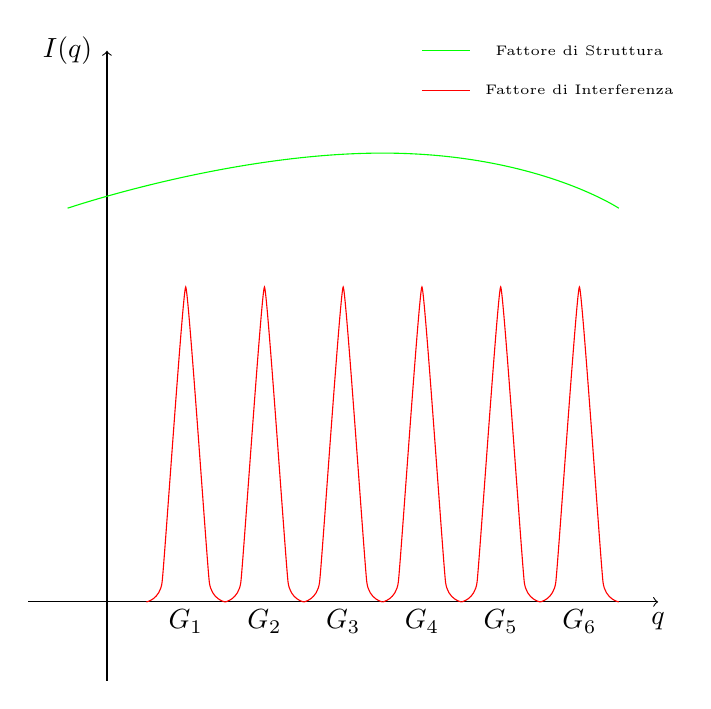
\begin{tikzpicture}[scale=1,auto=center]
			\draw [->] (-1,0) -- (7,0);
			\draw [->] (0,-1) -- (0,7);
			\node (n1) at (7,-0.25) {${\vet q}$};
			\node (n2) at (-0.5,7) {$I({\vet q})$};
			\node (n3) at (1,-0.25) {${\vet G_1}$};
			\node (n4) at (2,-0.25) {${\vet G_2}$};
			\node (n5) at (3,-0.25) {${\vet G_3}$};
			\node (n6) at (4,-0.25) {${\vet G_4}$};
			\node (n7) at (5,-0.25) {${\vet G_5}$};
			\node (n8) at (6,-0.25) {${\vet G_6}$};

			\draw [red] plot [smooth, tension=0.2] coordinates {(0.5,0) (0.7,0.25) (1,4) (1.3,0.25) (1.5,0)};
			\draw [red] plot [smooth, tension=0.2] coordinates {(1.5,0) (1.7,0.25) (2,4) (2.3,0.25) (2.5,0)};
			\draw [red] plot [smooth, tension=0.2] coordinates {(2.5,0) (2.7,0.25) (3,4) (3.3,0.25) (3.5,0)};
			\draw [red] plot [smooth, tension=0.2] coordinates {(3.5,0) (3.7,0.25) (4,4) (4.3,0.25) (4.5,0)};
			\draw [red] plot [smooth, tension=0.2] coordinates {(4.5,0) (4.7,0.25) (5,4) (5.3,0.25) (5.5,0)};
			\draw [red] plot [smooth, tension=0.2] coordinates {(5.5,0) (5.7,0.25) (6,4) (6.3,0.25) (6.5,0)};

			\draw [green] plot [smooth, tension=1] coordinates {(-0.5,5) (3.5,5.7) (6.5,5)};

			\draw [green] plot [smooth, tension=0] coordinates {(4,7) (4.6,7)};
			\draw [red] plot [smooth, tension=0] coordinates {(4,6.5) (4.6,6.5)};

			\node[] at (6,7) {\fontsize{1mm}{1mm}\selectfont Fattore di Struttura};
			\node[] at (6,6.5){\fontsize{1mm}{1mm}\selectfont Fattore di Interferenza};
		\end{tikzpicture}
	}
	\caption{Fattore di Interferenza e Fattore di Struttura}
	\label{str:int}
\end{figure}
In Fig.\ref{str:int} sono rappresentati i contributi dei fattori di interferenza e struttura. Come è possibile osservare il fattore di interferenza è rappresentato da dei picchi situati in prossimità dei vettori $ {\vet G_n}$ e identificano le $N$ celle del reticolo cristallino.
\subsection{Un Liquido}
Supponiamo di indebolire il fatto che il reticolo sia cristallino. Supponiamo di avere a che fare con un oggetto che abbia le caratteristiche di un fluido. In questo caso fisso un ${\vet R} _n$ e sommo su tutti i vari ${\vet R} _m$. Devo quindi avere una funzione di correlazione spaziale che mi permetta di sapere in che posizione sono i vari ${\vet R} _m$ ripetto al mio punto fisso ${\vet R} _n$. Il fattore di interferenza diventa quindi 
\newl{T({\vet q}) &=& \abs{\sum_{n_1,n_2,n_3} e^{-i{\vet q} \cdot{\vet R}_n } }^2 = \sum_{{\vet R}_m = {\vet R}_n} e^{-i{\vet q}\cdot({\vet R}_n -{\vet R}_m)}+ \sum_{{\vet R} _n \neq {\vet R} _m } e^{-i{\vet q} \cdot({\vet R} _n- {\vet R} _m)} = \nonumber\\ &=& N + \sum_{{\vet R_n}} \left(\sum_{{\vet R} _n \neq {\vet R} _m}e^{-i{\vet q}(\vet{R} _n - {\vet R} _m)} \right) }
Estendo al continuo
\newl{T(\vet{q}) &=& N + N\int d^3r\, e^{-i{\vet q}\cdot(R_n-R_m)}P(R_n-R_m) = \nonumber\\
			       &=& N\left(1+\int d^3r\, e^{-i{\vet q}\cdot(R_n-R_m)}P(R_n-R_m)\right) 
}
Dove $P(R_n-R_m)$ è la funzione di correlazione spaziale che permette di studiare strutture non perfettamente regolari.

